% Copyright (c) 2022 by Lars Spreng
% This work is licensed under the Creative Commons Attribution 4.0 International License. 
% To view a copy of this license, visit http://creativecommons.org/licenses/by/4.0/ or send a letter to Creative Commons, PO Box 1866, Mountain View, CA 94042, USA.

%~~~~~~~~~~~~~~~~~~~~~~~~~~~~~~~~~~~~~~~~~~~~~~~~~~~~~~~~~~~~~~~~~~~~~~~~~~~~~~
% You can add your packages and commands to the loadslides.tex file. 
% The files in the folder "styles" can be modified to change the layout and design of your slides.
% I have included examples on how to use the template below. 
% Some of these examples are taken from the Metropolis template.
%~~~~~~~~~~~~~~~~~~~~~~~~~~~~~~~~~~~~~~~~~~~~~~~~~~~~~~~~~~~~~~~~~~~~~~~~~~~~~~


\documentclass[
11pt,notheorems,hyperref={pdfauthor=whatever}
]{beamer}

\input{loadslides.tex} % Loads packages and some defined commands

\title[
% Text entered here will appear in the bottom middle
]{Anthropogenic Intensification of \\Short-Duration Rainfall Extremes}
\subtitle{Based on \citet{fowler2021}}


\author[
% Text entered here will appear in the bottom left corner
]{
    Nathasya Christien 
}

\institute{
    Earth System Modelling Course \\
    Earth System Physics Section \\
    The Abdus Salam International Centre for Theoretical Physics}
\date{\today}

\begin{document}

% Generate title page
{
\setbeamertemplate{footline}{} 
\begin{frame}
  \titlepage
\end{frame}
}
\addtocounter{framenumber}{-1}


\section{Introduction}

\begin{frame}
    \begin{block}{Motivation}
        \begin{itemize}
            \item Intensification of the hydrological cycle is a known effect of a warming climate, including rainfall extremes increase.
            \item Uncertainty remains in understanding changes to short-duration (1--3 h) and convective (tens of kilometers or less) events.
            \item Short-duration rainfall extremes are responsible for fatalities through flash floods and landslides.
        \end{itemize}
        
    \end{block}

    \begin{block}{Goals}
        \begin{itemize}
            \item Review observed trends and temperature-scaling studies, with insight from high-resolution climate models.
            \item Propose a conceptual framework to understand the intensification and its implications for flood risks.
            \item Address some gaps in the current knowledge.
        \end{itemize}
    \end{block}
\end{frame}

\section{Thermodynamics Baseline}

\subsection{Claysius-Clapeyron (CC) Relation}
\begin{frame}
    \begin{itemize}
        \item By (CC) relation, the saturation specific humidity of the atmosphere increases at a rate of $\sim7\%$ per degree warming near the Earth's surface.
        \item Given other atmospher conditions (e.g RH) remain constant across, the absolute (specific) humidity of air also increases at roughly the same rate.
        \item As rainfall extremes are limited by the amount of atmospheric moisture available, changes to rainfall intensities are expected to scale with the CC relation.
    \end{itemize}
\end{frame}

\subsection{Apparent and Climate Scaling}
\begin{frame}
    \begin{definition}
        \begin{itemize}
            \item Apparent scaling: Between extreme rainfall intensities and temperature from observed short-term climate variability.
            \item Climate scaling: How extreme rainfall will respond in a changing climate.
        \end{itemize}
    \end{definition}
\end{frame}

\begin{frame}
    \begin{columns}[onlytextwidth]
        \column{0.5\textwidth}
        \begin{itemize}
            \item Daily extremes mainly show apparent CC scaling.
            \item Super-CC scaling is observed in some locations for extreme hourly or shorter accumulations.
        \end{itemize}

        \column{0.5\textwidth}
        \centering
        {\scriptsize Temperature scaling of rainfall intensities for 10-min resolution}
        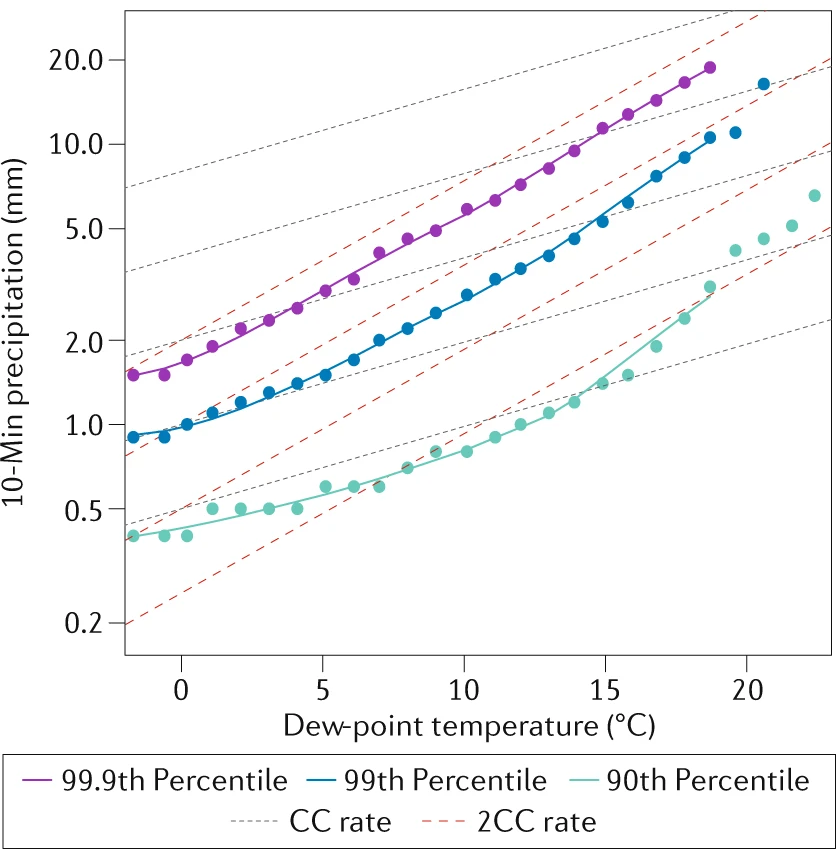
\includegraphics[width=0.8\textwidth]{./figs/fig2.png}
    \end{columns}
\end{frame}

\begin{frame}
    \begin{columns}[onlytextwidth]
        \column{0.5\textwidth}
        \begin{itemize}
            \item \textit{Apparent scaling depends on the temperature measurements used and the portion of the temperature range analysed.}
            \item Near-surface air temperature commonly produces CC or super-CC rates for hourly rainfall at 10--20°C, but negative rates at >20--25°C.
            \item Negative apparent scaling is explained by the drier conditions and the limited moisture availability on warm days, with high-pressure situations (high temperature, low RH).
            \item Including moisture in the assessment (e.g \textbf{dew-point temperature}) increases the consistency in apparent scaling.
            \item Understanding processes behind super-CC apparent scaling allow the exclusion of systematic dependencies irrelevant for climate scaling.
        \end{itemize}

        \column{0.5\textwidth}
        \centering
        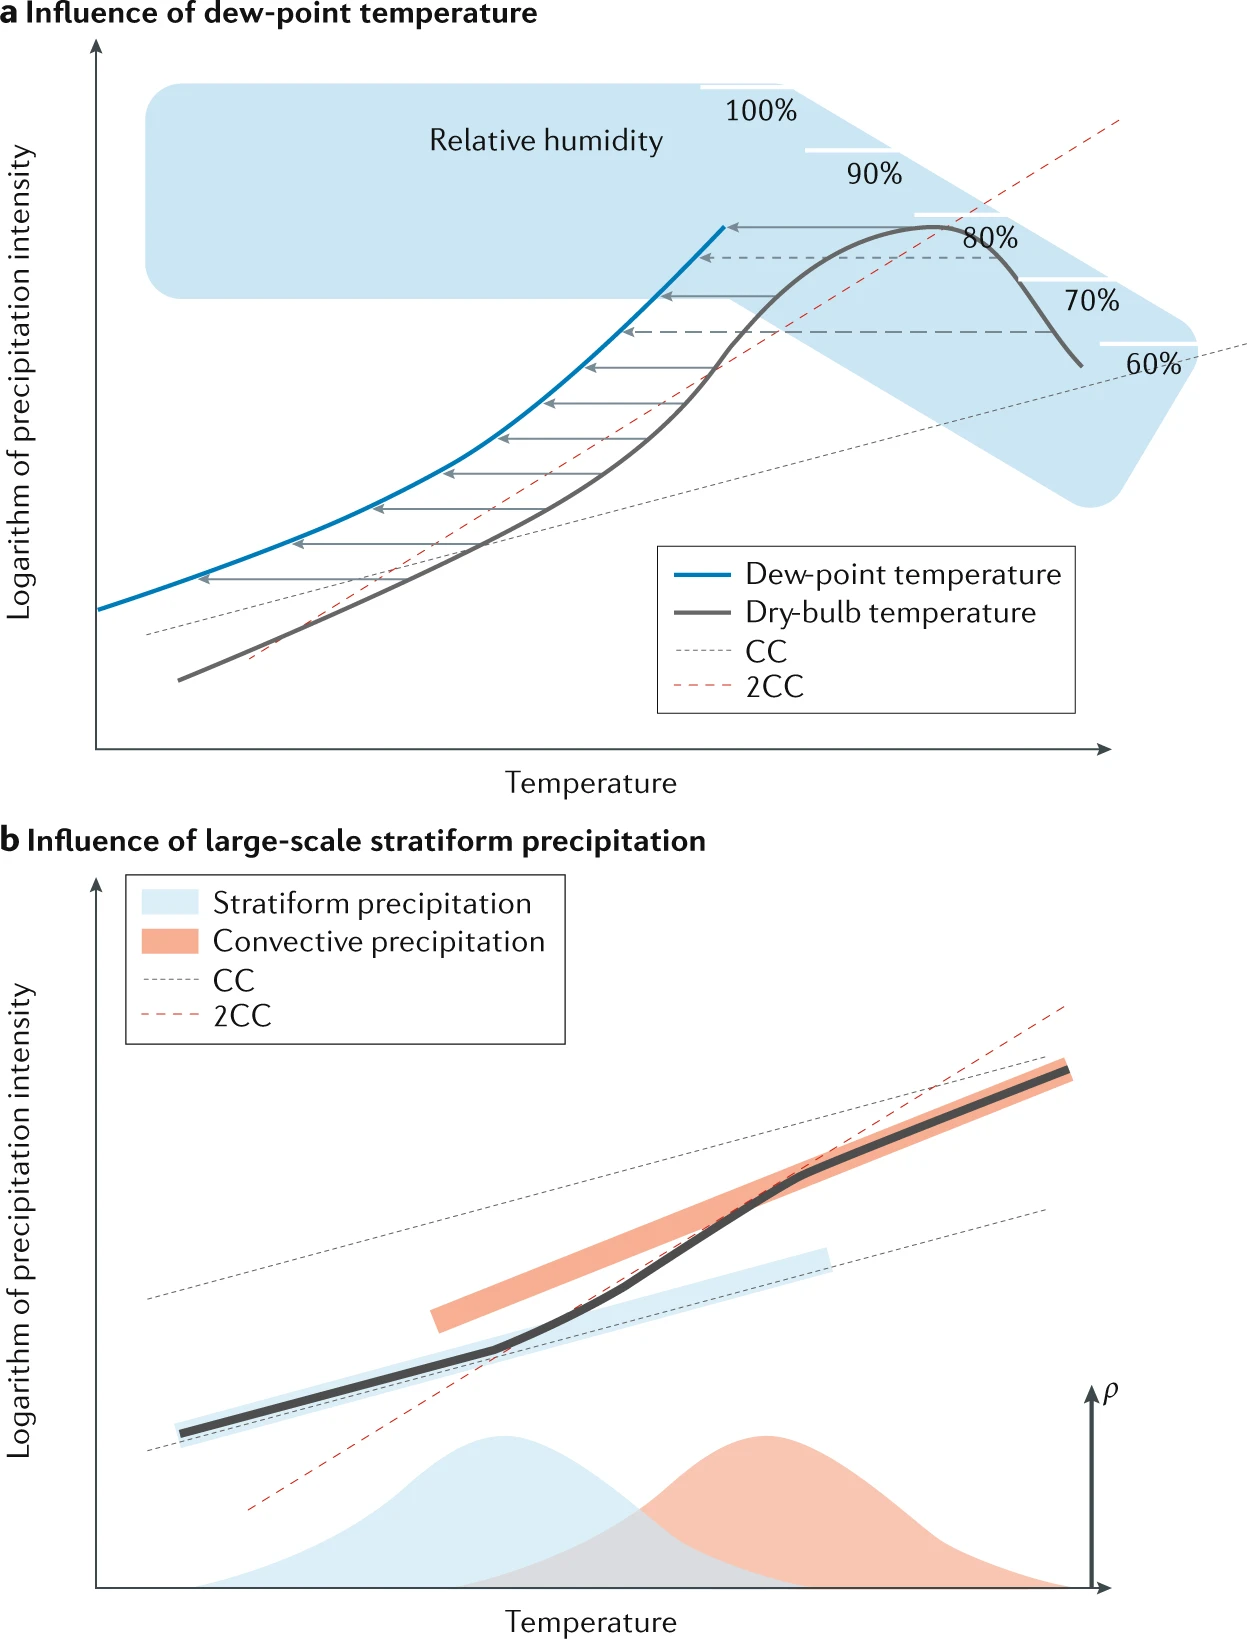
\includegraphics[width=0.8\textwidth]{./figs/fig3.png}
    \end{columns}
\end{frame}

% \begin{frame}
%     \begin{alertblock}{Caution in translating apparent scaling to climate scaling}
%         \begin{itemize}
%             \item Temperature scaling can be expected to be similar for short-term variability and future warming when sampling consistent meteorological regimes and by considering the influence of moisture and latent heat release.
%             \item Changes to temperature stratification in the atmosphere and to large-scale (or mesoscale) circulation variability should be assessed seperately. 
%         \end{itemize}
%     \end{alertblock}
% \end{frame}

\section{Changes in Sub-Daily Rainfall Extremes}
\subsection{Observational Trends}

\begin{frame}
    \centering    
    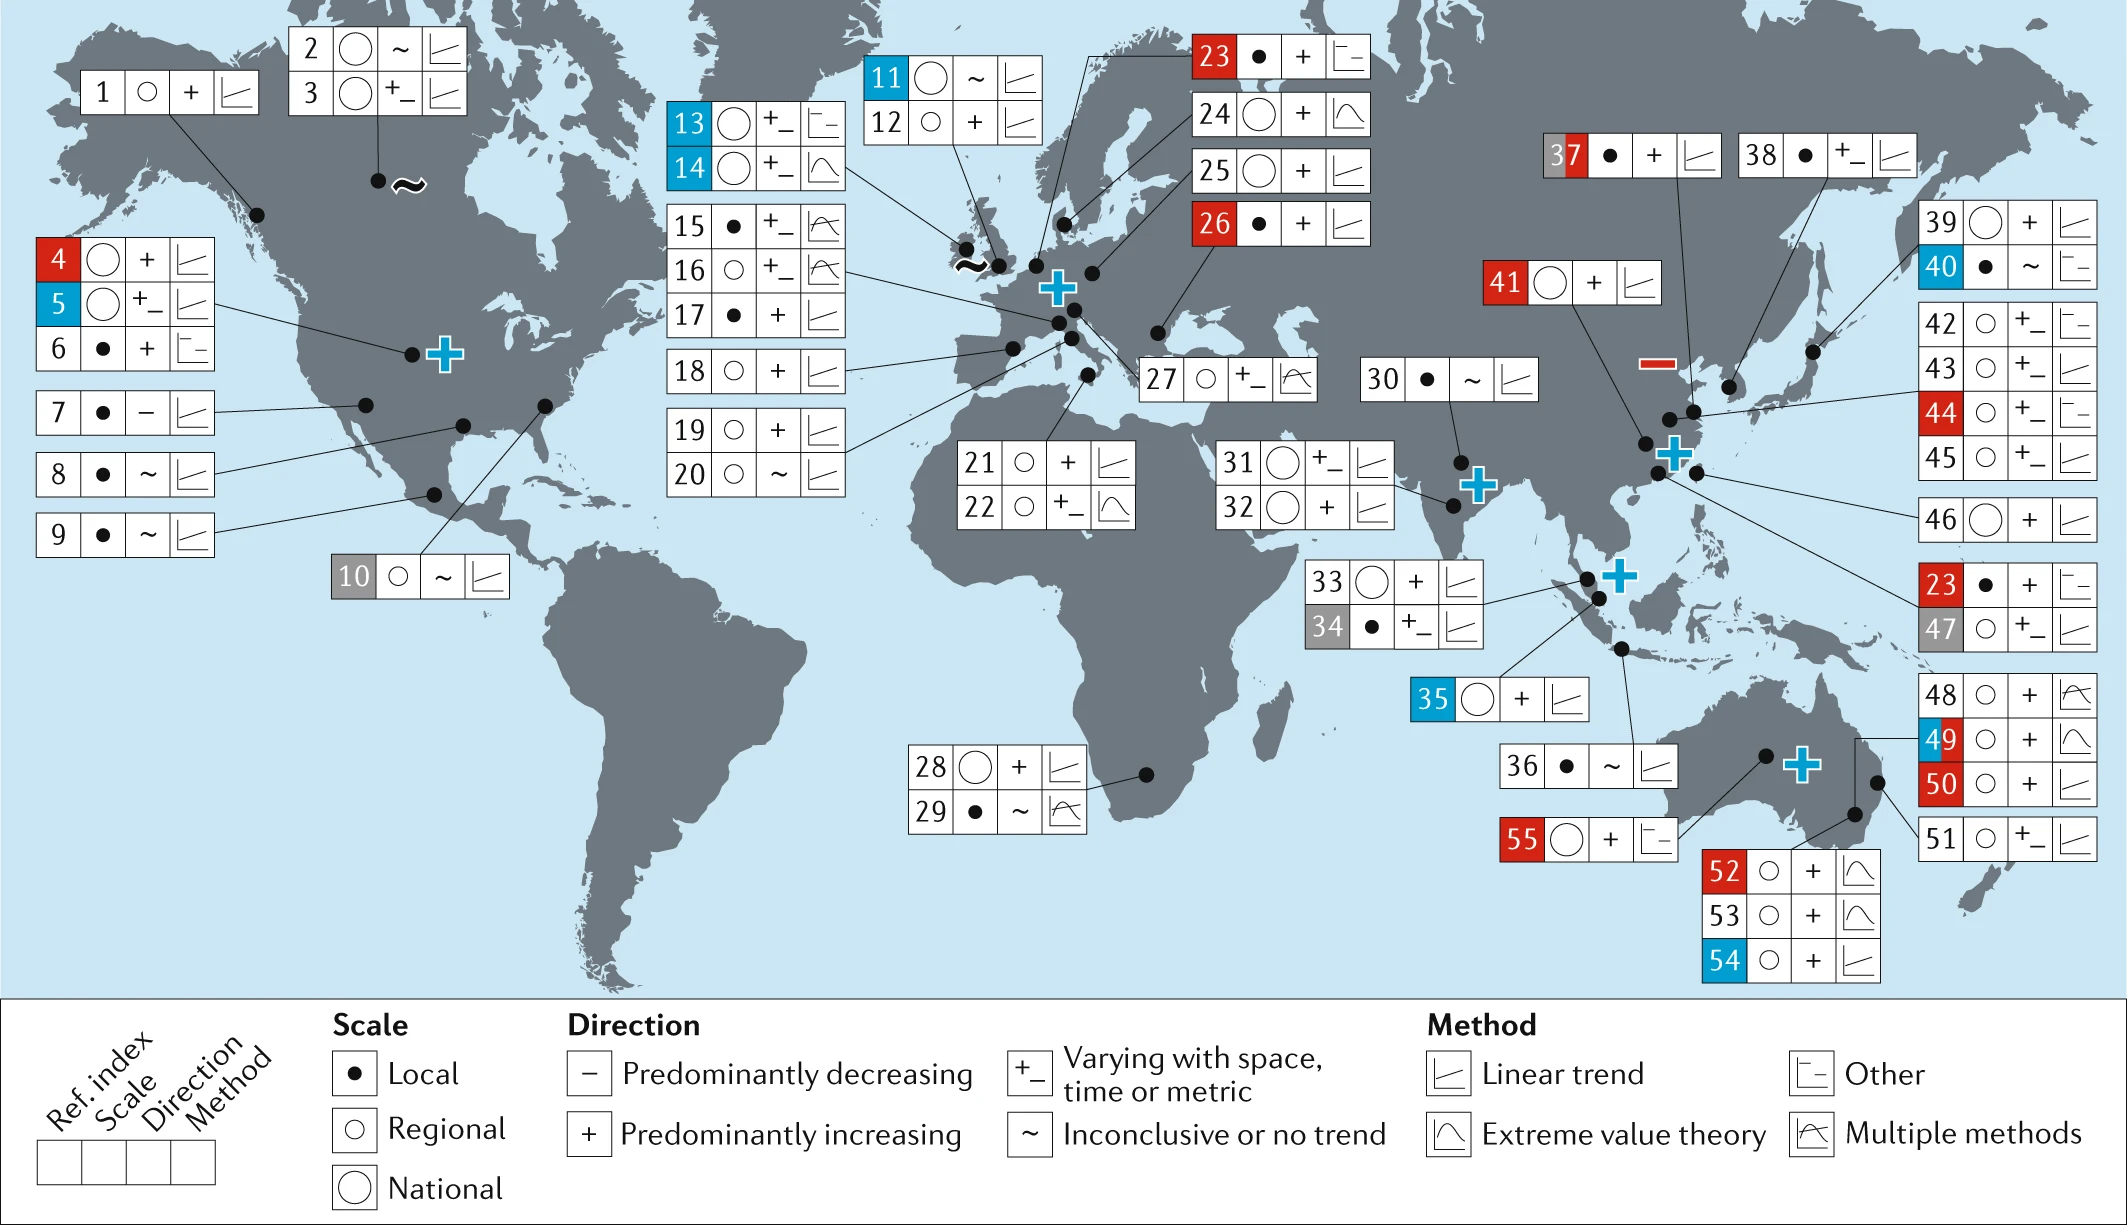
\includegraphics[width=0.8\textwidth]{./figs/fig4.png}

    \vspace{0.2cm}
    {\scriptsize Existing knowledge of observed changes in the frequency and/or intensity of sub-daily rainfall extremes}
\end{frame}


\subsection{Findings from Convective Permitting Models (CPMs)}
\begin{frame}
    \begin{itemize}
        \item Traditional climate models use parameterizations for deep convection, missing the spatial details of convective motions.
        \item CPMs use grid spacing <5 km, allowing them to explicitly resolve cloud dynamical processes.
        \item CPMs consistently project higher intensification of sub-daily extremes (at or above CC) compared to coarser models.
    \end{itemize}
\end{frame}

\subsection{Storm Track Changes}
\begin{frame}
    \begin{itemize}
        \item Some studies show storms becoming smaller but more intense (Australia/Germany), while others show both intensity and spatial size increasing (Netherlands).
        \item An increase in both peak intensity and spatial footprint (storm size) can result in massive increases in total "event" rainfall.
    \end{itemize}
\end{frame}


\section{Physical Mechanisms}
\begin{frame}
    \centering
    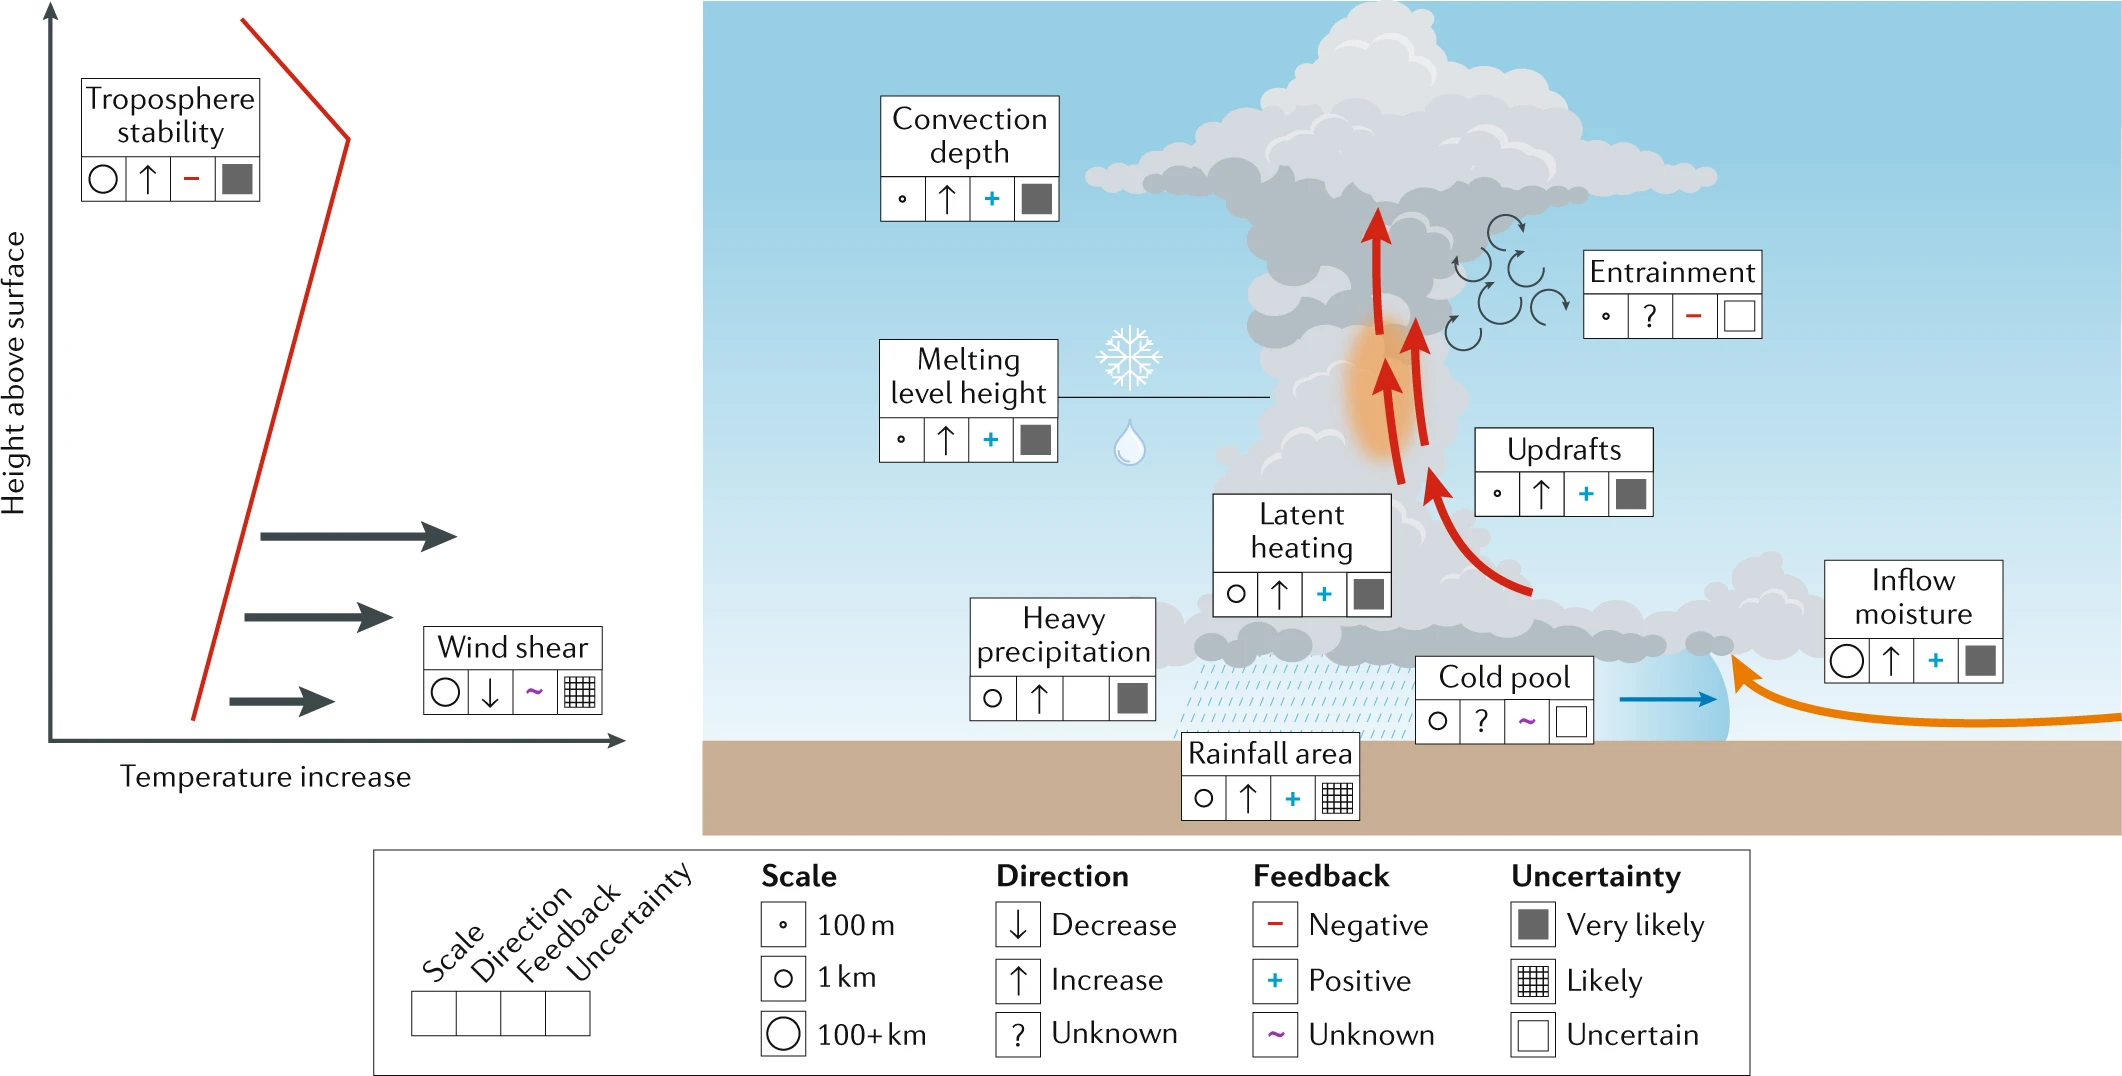
\includegraphics[width=0.9\textwidth]{./figs/fig5.png}

    \vspace{0.2cm}
    {\scriptsize Climate change-induced changes in extreme convective sub-daily precipitation processes}
\end{frame}


\section{Implications for Flood Hazards}
\begin{frame}
    \centering
    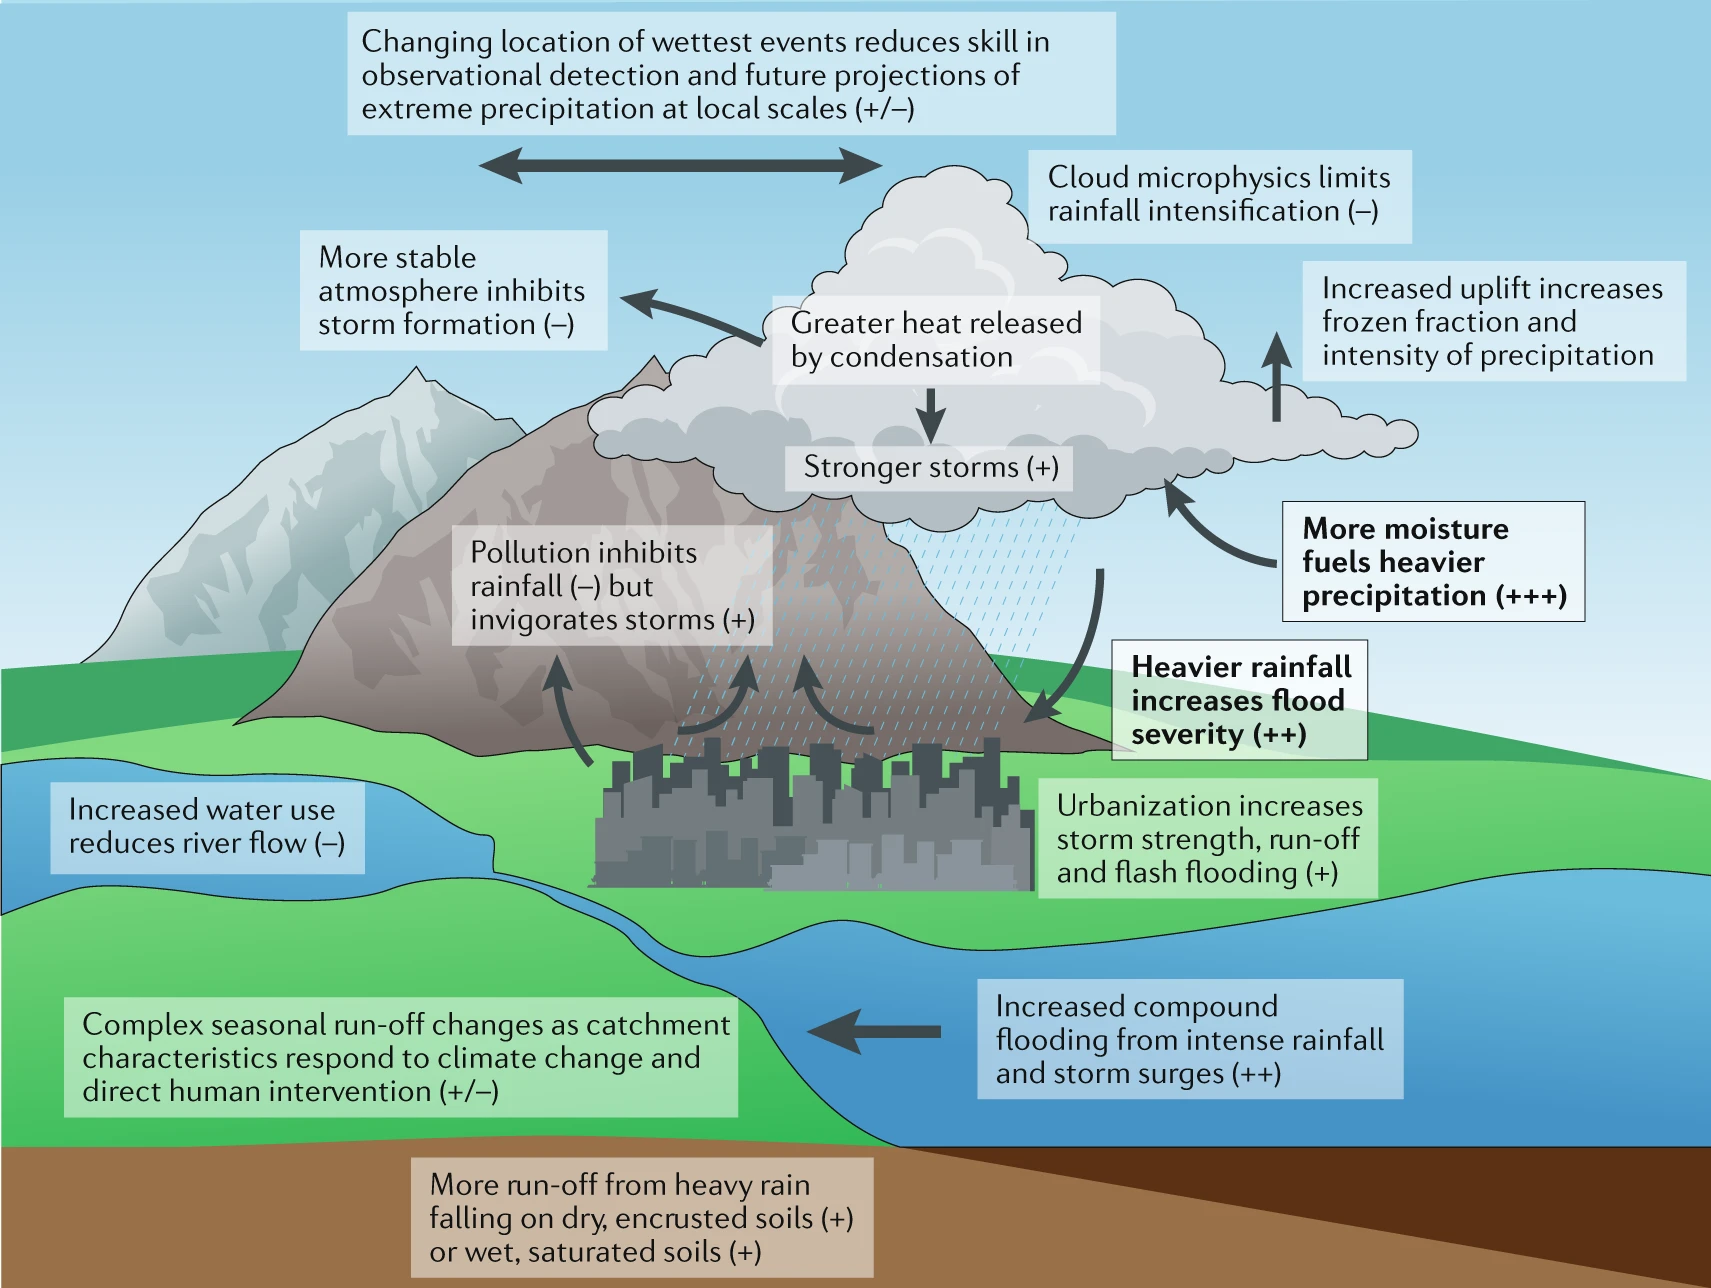
\includegraphics[width=0.7\textwidth]{./figs/fig6.png}

    \vspace{0.2cm}
    {\scriptsize Changes in sub-daily precipitation extremes and the flood hazard}
\end{frame}

\section{Conclusion}
\begin{frame}
    \begin{itemize}
        \item Short-duration extremes are intensifying at CC or super-CC rates due to thermodynamic and dynamical feedbacks.
        \item There is an urgent need for climate-resilient engineering and adaptation measures, especially in urban areas, to manage the non-linear increase in flood risk.
    \end{itemize}
\end{frame}


% \begin{frame}[allowframebreaks]{References}
%     \printbibliography
% \end{frame}
\end{document}